% ------------------------------------------------------------------------
% ------------------------------------------------------------------------
% Atualizado para as citações - (SILVA, 2023) para (Silva, 2023)  de acordo com a NBR 10520/2023 
% ------------------------------------------------------------------------

\documentclass[a4paper, portugues,11pt]{article}
\usepackage[brazilian]{babel}

\usepackage[utf8]{inputenc}
\usepackage[scaled]{berasans} %https://tug.org/FontCatalogue/berasans/
\renewcommand*\familydefault{\sfdefault}  %% Não encontrei a spranq eco sans para Latex, a Bera Sans é igual mas sem os furinhos
\usepackage[T1]{fontenc}
%\usepackage[latin1]{inputenc}

\usepackage{lipsum} % texto aleatório em latim

\usepackage{url}
\usepackage{setspace}

\usepackage{enumerate} % para os dois tipos de listas

\usepackage{multicol}
%\usepackage{isolatin1}
%\usepackage[dvips]{graphicx}

\usepackage[pdftex]{graphicx}
\usepackage[pdftex]{hyperref}
\usepackage[pdftex]{color}

\usepackage[dvipsnames]{xcolor}
%\usepackage{color}				% Controle das cores

\usepackage{pifont} %símbolos marcadores
\usepackage{nomencl} % Lista de simbolos
\usepackage[normalem]{ulem} %sublinhados
%simbolos marcadores
\usepackage{amssymb}
\usepackage{indentfirst}
\usepackage{setspace}
\usepackage{graphicx}			% Inclusão de gráficos
\usepackage{microtype} 			% para melhorias de justificação

\usepackage{zref-totpages} %calcula o total de páginas

\usepackage[
    bottom=2cm,
    top=1cm,
    left=2.5cm,
    right=1.5cm, 
    headsep=1.5cm,
    %headheight=14.5pt, %%% 3mm is too small
    %heightrounded
    includehead, 
    includefoot
    ]{geometry}


% \hyphenation{se-ma-na}

\onehalfspacing
%\singlespace

%------------------------------------------------------------------------

% Seleciona o idioma do documento (conforme pacotes do babel)
%\selectlanguage{english}

% ---
% PACOTES
% ---

% ---       
% Pacotes fundamentais 
% ---
%\usepackage{lmodern}			% Usa a fonte Latin Modern
%\usepackage{mathptmx} % Fonte times new romam no texto
%\usepackage{ccfonts}




		
% ---
% Pacotes de citações
% ---

\usepackage[alf]{abntex2cite}	% Citações padrão ABNT
% ---


% alterando o aspecto da cor azul
\definecolor{blue}{RGB}{41,5,195}

\makeatother
% --- 


%\usepackage{fancyhdr} %cabeçalhos
\usepackage{fancyhdr,xpatch}
\fancyhf{} % limpa os cabeçalho e rodapés
\pagestyle{fancy} % sem definir esse comando, o cabeçalho personalizado não é exibido

\fancyhead{} % define o cabeçalho personalizado
\renewcommand{\headrulewidth}{0mm}
\lhead{}
\chead{}
\rhead{}

\fancyfoot{}
\renewcommand{\footrulewidth}{0mm}
\lfoot{}
\cfoot{}
\rfoot{\thepage}



% ----
% Configurar primeiras seções e sumário

\makeatletter
\let\ORI@section\section
\renewcommand{\section}{\@ifstar\s@section\ORI@section}
\newcommand{\s@section}[1]{%
  \ORI@section*{#1}
  \csname phantomsection\endcsname % for hyperref
  \addcontentsline{toc}{section}{#1}
}
\xpatchcmd{\tableofcontents}{\section}{\ORI@section}{}{} % toc not in toc
\makeatother

% ----
\begin{document}

\newgeometry{top=20mm, bottom=20mm, right=20mm, left=20mm}
\thispagestyle{empty}

\begin{figure}[!htbp]
  \begin{center}
    
\includegraphics[angle=0, width=0.91\textwidth]{Imagens/capa-ps.jpg}
  \end{center}
 \end{figure}

 \begin{center}
  {\huge Modelo em \LaTeX \ para o Prêmio SERPRO} \\
  \vspace{30mm}
  {\Large Weldson Queiroz de Lima} \\
  \vspace{30mm}
  {\Large Tema: Altruísmo acadêmico e corporativo} \\
  {\Large \vfill Nº de páginas: \ztotpages} \\
	%\textbf{\LARGE Modelo em \LaTeX para o Prêmio Serpro}
\end{center}

\restoregeometry % 
\clearpage
\pagenumbering{arabic}
\section*{Folha de Rosto}

\hspace*{-6.5mm} \underline{Título do Trabalho:} Modelo em \LaTeX \ para o Prêmio SERPRO \\ 
\vspace{10mm}

\hspace*{-6.5mm} \underline{Tema:} Altruísmo acadêmico e corporativo \\ 
\vspace{10mm}

\hspace*{-6.5mm} \underline{Autores:} Weldson Queiroz de Lima \\ 
\vspace{10mm}

\hspace*{-6.5mm} \underline{Curriculos:} Possui graduação em Tecnologia em Informática pelo Centro Federal de Educação Tecnológica do Rio Grande do Norte (CEFET-RN), especialização em Gestão Pública pela Universidade Federal do Rio Grande do Sul (UFRGS), MBA em Gestão Pública pela Escola Nacional de Administração Pública (ENAP) e mestrado em Engenharia Elétrica pela Universidade Federal do Rio Grande do Norte (UFRN). Atualmente é gestor de departamento de Inteligência, Estratégia e Qualidade dos Produtos e Serviços de Operação no Serviço Federal de Processamento de Dados (SERPRO). Em acumulação, é docente do Instituto Federal de Educação, Ciência e Tecnologia de Brasília, onde desenvolve atividades acadêmicas relacionadas a tecnologia e governo digital.  \\ 
\vspace{10mm}

\clearpage
\section*{Resumo}
\lipsum[1]

\vspace{10mm}
\hspace*{-6.5mm} \underline{Palavras-chaves:} Serpro; \LaTeX; Prêmio. \\ 

\clearpage
\listoffigures

\clearpage
\tableofcontents

%\clearpage
%\listoftables 

\clearpage
% Retira espaço extra obsoleto entre as frases.
\frenchspacing 


%\setcounter{section}{3}
\section{Introdução}
  \lipsum[1] \\

\section{Referencial Teórico}

\lipsum[2] 

\begin{figure}[!htbp]
  \begin{center}
    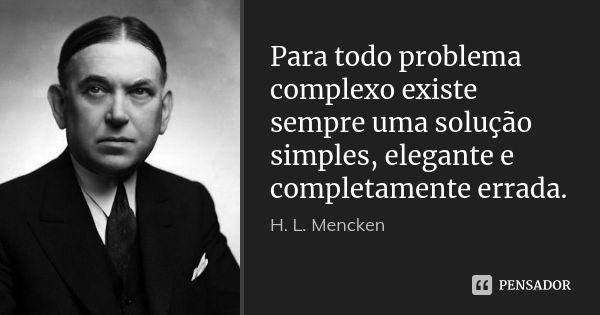
\includegraphics[angle=0, width=0.6\textwidth]{Imagens/h_l_mencken.jpg}
  \caption{Wicked Problems \label{fig:rg}}
  \end{center}
 \end{figure}


Minha pesquisa, fundamentada na figura \ref{fig:rg}, durante o mestrado na UFRN e na RNP foi focada em protocolos de rede e roteamento IP Multicast \cite{weldsonufrn}. Nos anos seguintes os resultados da pesquisa foram aplicados em atividades de ensino, docência e publicados em periódicos internacionais relevantes \cite{weldson2004} \cite{DBLP:conf/policy/FrancoLSPATGBJF06} \cite{DBLP:conf/noms/LimaAVATG06}. 

\section{Metodologia}

\lipsum[2]
Dar preferência às questões práticas que envolvem a área de atuação profissional do candidato. Figura \ref{fig:soap} apresenta o esqueleto de uma mensagem SOAP. O \texttt{soap:Envelope} é o elemento raiz do documento XML.

\begin{figure}[!htbp]
 \begin{center}
 \begin{tabular}[htb]{|c|}
 \hline
 \begin{minipage}[b]{0.8\linewidth}
 \vspace*{2mm}
 \texttt{\footnotesize
{\color{Gray}\footnotesize \ 01. }<?xml version="1.0"?> \\
{\color{Gray}\footnotesize \ 02. }<soap:Envelope \\
{\color{Gray}\footnotesize \ 03. }xmlns:soap=``http://www.w3.org/2001/12/soap-envelope'' \\
{\color{Gray}\footnotesize \ 04. }soap:encodingStyle=``http://www.w3.org/2001/12/soap-encoding''> \\
{\color{Gray}\footnotesize \ 05. }\hspace{5mm}<soap:Header> \\
{\color{Gray}\footnotesize \ 06. }\hspace{10mm}... \\
{\color{Gray}\footnotesize \ 07. }\hspace{5mm}</soap:Body> \\
{\color{Gray}\footnotesize \ 08. }</soap:Envelope> \\
   }
 \end{minipage}
 \\ \hline
 \end{tabular}
 \caption{Exemplo de mensagem SOAP \label{fig:soap}}
 \end{center}
\end{figure}

\section{Lacuna de conhecimento aplicado}

\lipsum[2]

\begin{itemize}
  \item[\ding{51}] Code 51
  \item[\ding{52}] Code 52
  \item[\ding{54}] Code 54
  \item[\ding{55}] Code 55
  \item[\ding{212}] Code 212
  \item default
\end{itemize}

\lipsum[1] 

\begin{enumerate}
  \item One
  \item Two
  \item Three
\end{enumerate}

\section{Inferência de resultado em escala}

\lipsum[2] 


\begin{table}[htb]
  \begin{center}
  \begin{tabular}{|l|l||c|c|c|c|c|c|c|}
  \hline
  \multicolumn{2}{|c|}{\bf Dia} & \multicolumn{2}{|c|}{\bf Manhã} & \multicolumn{2}{|c|}{\bf Tarde} & \multicolumn{2}{|c|}{\bf Noite} & {\bf Total} \\ \cline{3-9}
  \multicolumn{2}{|c|}{\bf }  & {\bf \ E \ } & {\bf \ S \ } & {\bf  \ E \ } & {\bf \ S \ } & {\bf \ E \ } & {\bf \ S \ } & {\bf hs} \\
      \hline \cline{1-09}
  
  {\bf 01} & {\bf Domingo} & \colorbox{Gray}{\hspace{6mm}} & \colorbox{Gray}{\hspace{6mm}} & \colorbox{Gray}{\hspace{6mm}} & \colorbox{Blue}{\hspace{6mm}} & \colorbox{Gray}{\hspace{6mm}} & \colorbox{Gray}{\hspace{6mm}} & \colorbox{Gray}{\hspace{9mm}}  \\ \hline 
  {\bf 02} & {\bf Segunda} &  &  &  &  & - & - &   \\ \hline
  {\bf 03} & {\bf Terça} &  &  &  &  &  - & - &  \\ \hline 
  {\bf 04} & {\bf Quarta} &  &  &  &  &  - & - &  \\ \hline  
  {\bf 05} & {\bf Quinta} &  &  &  &  &  - & - &  \\ \hline
  {\bf 06} & {\bf Sexta} &  &  &  &  &  - & - &  \\ \hline
  {\bf 07} & {\bf Sábado} & \colorbox{Gray}{\hspace{6mm}} & \colorbox{Gray}{\hspace{6mm}} & \colorbox{Gray}{\hspace{6mm}} & \colorbox{Gray}{\hspace{6mm}} & \colorbox{Gray}{\hspace{6mm}} & \colorbox{Gray}{\hspace{6mm}} & \colorbox{Gray}{\hspace{9mm}}  \\ \hline 
  {\bf 08} & {\bf Domingo} & \colorbox{Gray}{\hspace{6mm}} & \colorbox{Gray}{\hspace{6mm}} & \colorbox{Gray}{\hspace{6mm}} & \colorbox{Gray}{\hspace{6mm}} & \colorbox{Gray}{\hspace{6mm}} & \colorbox{Gray}{\hspace{6mm}} & \colorbox{Gray}{\hspace{9mm}}  \\ \hline 
  {\bf 09} & {\bf Segunda} &  &  &  &  &  18:00 & 22:00 &  4:00 \\ \hline \cline{1-09}
  % {\bf 15} & {\bf Terça} & X & X & X & X & X & X & FERIADO & X \\ \hline 
  % {\bf 29} & {\bf Sábado} &  &  &  &  \colorbox{Gray}{\hspace{6mm}}  &  &  &  &  \\ \hline \cline{1-10}
  \multicolumn{8}{|r|}{\bf Total de horas presenciais no mês \ \ } & 64:00 \\ \hline
  \end{tabular}
  \caption{Tabela complexa} \label{tab:comp}
  \end{center}
  \end{table}


\section{Conclusão} \label{sec:obj}
  \lipsum[10] 


\clearpage
% ----------------------------------------------------------
% Referências bibliográficas
% ----------------------------------------------------------
\bibliographystyle{tex/abntex2-alf.bst}
\bibliography{abntex2-references}

% ----------------------------------------------------------
% Glossário
% ----------------------------------------------------------
%
% Há diversas soluções prontas para glossário em LaTeX. 
% Consulte o manual do abnTeX2 para obter sugestões.
%
%\glossary

% ----------------------------------------------------------
% Apêndices
% ----------------------------------------------------------

% ---
% Inicia os apêndices
% ---

% ---

% ----------------------------------------------------------
% Anexos
% ----------------------------------------------------------

% ----------------------------------------------------------
% Agradecimentos
% ----------------------------------------------------------



\end{document}
